%!TEX program = xelatex
%!TEX TS-program = xelatex
%!TEX encoding = UTF-8 Unicode

\documentclass[12pt, a4paper]{article}
\usepackage{CJKutf8}
\usepackage{graphicx}
\usepackage{subfigure}
\usepackage{listings}
\usepackage[colorlinks,linkcolor=blue]{hyperref}
\usepackage{ulem}
\usepackage{xcolor}
\usepackage{caption2}
\usepackage{amssymb}
\usepackage{indentfirst} % 中文段落首行缩进
\setlength{\parskip}{0.5em}
\renewcommand{\figurename}{图} % 将图表的标题设置为中文“图”

\title{第十六·承诺博弈 · 有效承诺方能赢得合作}
\author{hoochanlon}
\date{\today}

\begin{document}
	\begin{CJK*}{UTF8}{gbsn}
		\maketitle
        \clearpage
        \section{承诺与威胁}
        静态博弈中,一般不存在承诺和威胁。动态博弈则不同,后行动者可以提前给先行动者一个承诺或威胁,对后续的行动选择给出某种保证,
        从而期望改变先行动者的行动。
        \begin{itemize}
            \item 一般来说,承诺是给对方有利的行动,那我们叫胡萝卜模式。
            \item 威胁或给出对方不利行动,我们叫他大棒模式。
        \end{itemize}
        \subsection{可信承诺与可信威胁}
        \subsubsection{可信性}
        \begin{itemize}
            \item 可信性是指博弈中先行动的参与者是否该相信后行动的参与者会采取对自己有利的或不利的行为。
            \item 后行动者将来会采取对先行动方有利的行为相当于一种“承诺”;而将来会采取对先行为方不利的行为相当于一种“威胁”。
            \item 可信性分为“承诺的可信性”和“威胁的可信性”,即可信承诺和可信威胁。
        \end{itemize}
        \subsubsection{可信承诺}
        可信承诺,事前事中都是有效的,对方在事中也认为是值得执行的,是符合序贯理性的承诺。轮到后行动者采取行动的时候,那么他出于自身利益的考虑,
        他确实会按照先前所声明的方式来参与行动。要想让先行动者相信自己的承诺,就有两种具体方法:
        \begin{enumerate}
            \item 减少未来行动的自由或可能性。比如:破釜沉舟,把船都整没了,没有退路了。
            \item 改变未来的损益。比如:抵押贷款,如果不还钱,就会失去抵押品,未来损失更大。
        \end{enumerate}
        \clearpage
        \section{皇帝与功臣的博弈}
        皇帝:虽然我不知道你想不想谋反,但我知道你有没有能力来谋反,那些没能力的,心有余力而不足。

        \begin{figure}[htbp]
            \centering
			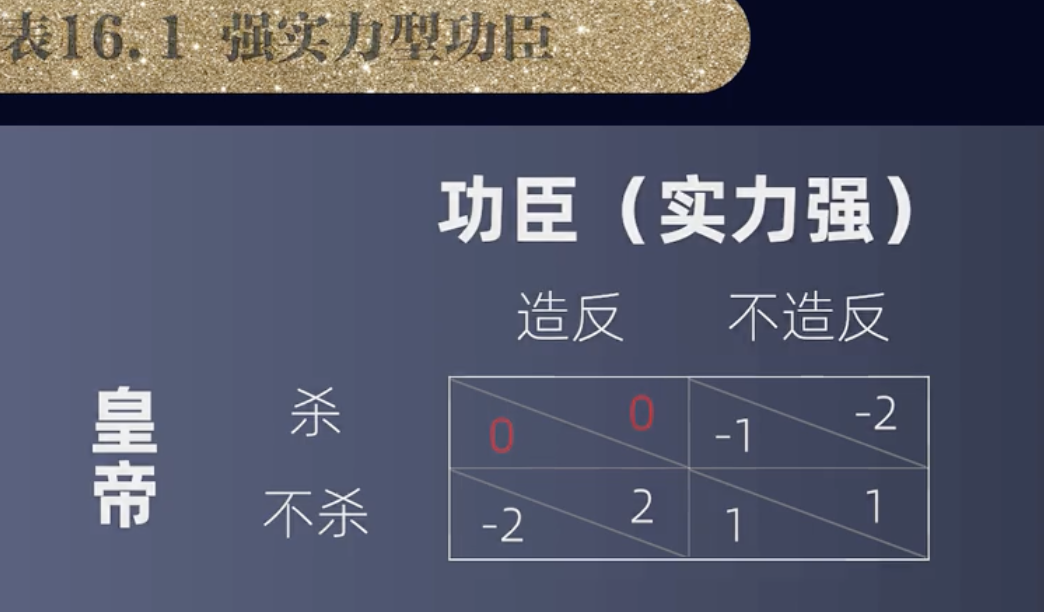
\includegraphics[width=0.6\textwidth]{./figures/catch2023-08-01-23.30.50.png}
            \caption{功臣实力强的博弈形态及结果}
        \end{figure}

        \begin{figure}[htbp]
            \centering
			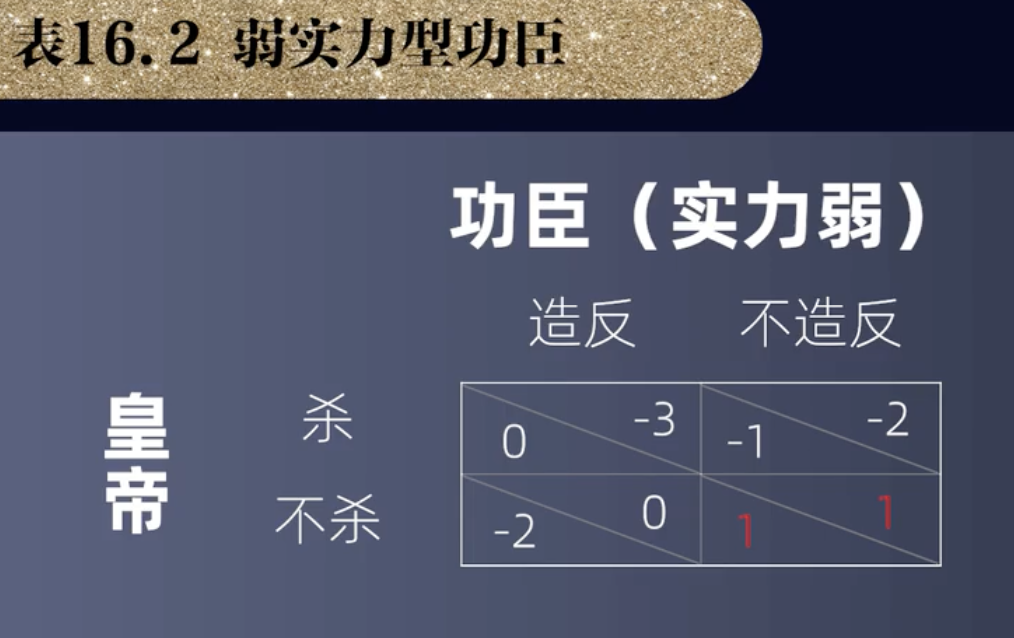
\includegraphics[width=0.6\textwidth]{./figures/catch2023-08-01-23.40.21.png}
            \caption{功臣实力弱的博弈形态及结果}
        \end{figure}

        功臣实力强的,保住性命又想有后续发展:告老还乡、自污其名、自杀身亡(规避满门抄斩)

        \clearpage
        \section{减肥博弈}
        减肥博弈模型:现在的你 VS 未来的你。

        \begin{figure}[htbp]
            \centering
			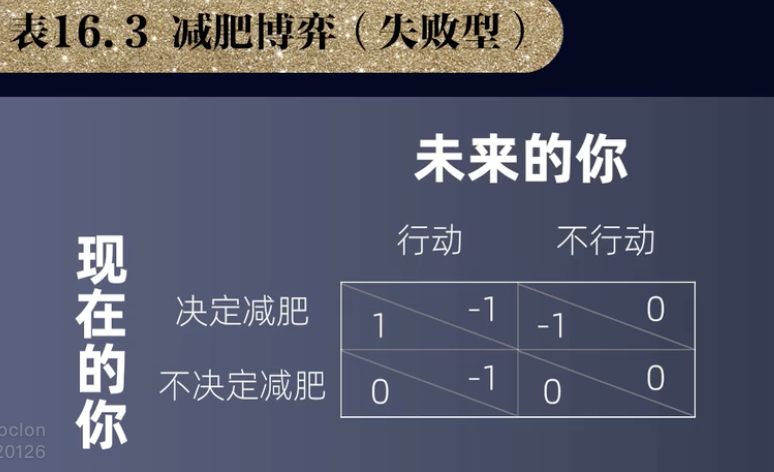
\includegraphics[width=0.6\textwidth]{./figures/catch2023-08-02-00.01.50.png}
            \caption{减肥博弈形态及结果}
        \end{figure}

        昨天的你下决心减肥,今天的你决定先满足当下的口腹之欲,晚饭以后继续重复昨天的故事,周而复始。最后的博弈结果:是现在的你不再决定减肥,
        未来的你也不再纠结于要不要吃晚饭。减肥失败的原因:不行动对未来的损益无影响。

        \begin{figure}[htbp]
            \centering
			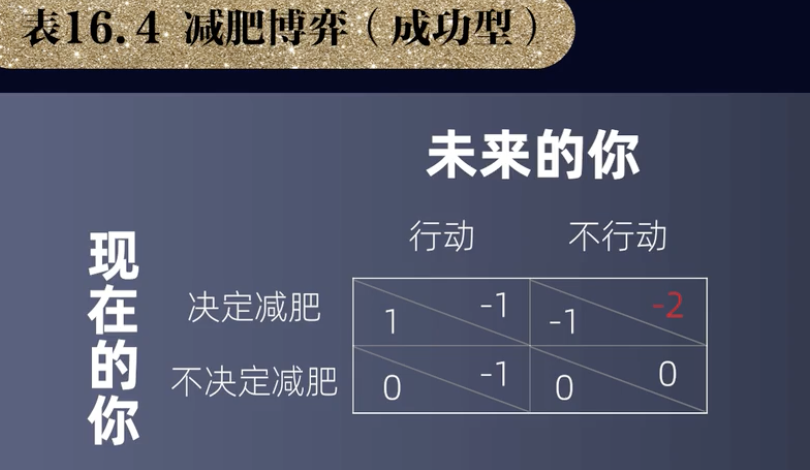
\includegraphics[width=0.6\textwidth]{./figures/catch2023-08-02-00.09.24.png}
            \caption{改变未来损益后的减肥博弈形态及结果}
        \end{figure}

        通过改变对未来自己的激励,从而改变未来自己的行为。很多人以为有更多的选择,就会让我们变得更好,但其实在博弈论中的思维是这样的:
        去掉一些选项,反而会让你做的更好。

    \end{CJK*}
\end{document}
